% !TEX program = pdflatex+makeindex+bibtex
% !TEX encoding = UTF-8 Unicode
% !TEX spellcheck = de_ch

% created by Simon Schälli <simon.schaelli@kantiwattwil.ch>
% v1.0 ursprüngliche Version
% v1.1 2015-10-22 mit Titelbild
% v1.2 2016-09-30 aufgeräumt
% v1.3 2016-10-16 Layoutfehler behoben

%======================================================================%
%=== Dokument auf häufige Fehler überprüfen                         ===%
%======================================================================%
\RequirePackage[l2tabu, orthodox]{nag}

%======================================================================%
%=== Dokumentklasse wählen                                          ===%
%======================================================================%
\documentclass[a4paper,twoside,openright]{scrreprt}

%======================================================================%
%=== Pakete einbinden                                               ===%
%======================================================================%
\usepackage[utf8]{inputenc}
\usepackage[ngerman]{babel}

% Latin Modern Schriftart
\usepackage{lmodern}
\usepackage[T1]{fontenc}

% Mathematik-Pakete
\usepackage{amsmath}
\usepackage{amssymb}

% mathematische Buchstaben als Text
\usepackage{textcomp}

% komfortable Referenzen mit \fref
\usepackage[german]{fancyref}

% Kopf- und Fusszeilen
\usepackage[automark,headsepline]{scrpage2}
\ihead[]{\headmark}
\chead[]{}
\ohead[]{\pagemark}
\ifoot[]{}
\cfoot[\pagemark]{}
\ofoot[]{}
\pagestyle{scrheadings}

% Einfügen von Bildern
\usepackage{graphicx}

% schöne Tabellen
\usepackage{booktabs}

% Tabelleninhalt an Dezimalpunkt ausrichten
\usepackage{dcolumn}
\makeatletter                     % <- hebt Sonderbedeutung von @ auf
\newcolumntype{d}[1]{D{.}{.}{#1}} % <- definiert einen neuen Spaltentyp
\makeatother                      % <- setzt Sonderbedeutung von @ wieder

% Beispieltext
\usepackage{lipsum}

% Hyperlinks in PDF
\usepackage{hyperref}

%======================================================================%
%=== Angaben zum Dokument                                           ===%
%======================================================================%

\titlehead{Kantonsschule Wattwil \hfill Hans Muster\\
Fachschaft Freizeit \hfill Musterweg 42\\
Näppisuelistrasse 11 \hfill 9999 Nirgendwo\\
9630 Wattwil}
\subject{Maturaarbeit}
\title{Meine Maturaarbeit}
\subtitle{Untertitel der Arbeit}
\author{\texorpdfstring{Hans Muster\\[1cm]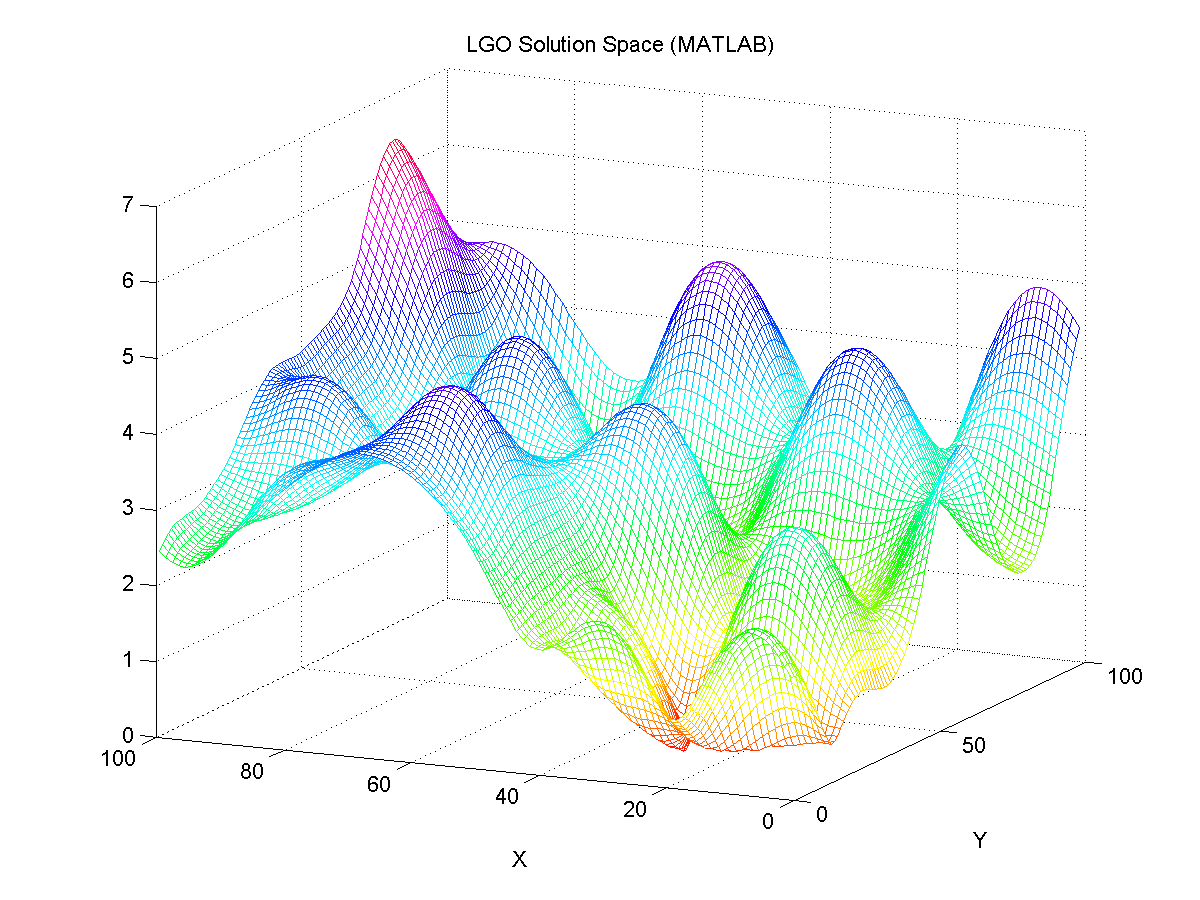
\includegraphics[scale=0.2]{figures/matlabgraph}\\[1cm] {\small Betreuer: Lehrer Beispiel}}{Hans Muster}}
\date{\small xx.xx.20xx}
%======================================================================%
%=== PDF Dokumenteinstellungen                                      ===%
%======================================================================%

\makeatletter
\hypersetup{
	pdftitle={\@title},%
	pdfsubject={\@subject},%
	pdfauthor={\@author},%
	pdfkeywords={},%
	colorlinks,%
	citecolor=black,%
	filecolor=black,%
	linkcolor=black,%
	urlcolor=black}%
\makeatother

%======================================================================%
%=== Beginn des eigentlichen Dokumentes                             ===%
%======================================================================%

\begin{document}

\maketitle % <- Titel setzen
\cleardoublepage
\pagenumbering{roman} % <- römische Seitennummerierung
\tableofcontents % <- Inhaltsverzeichnis
\cleardoublepage % <- neue Seite
\pagenumbering{arabic} % <- arabische Seitennummerierung

% Kapitel einbinden:
% !TEX root = ../maturaarbeit.tex
\chapter{Vorwort}\label{chap:vorwort}
\begin{enumerate}
\item Weshalb haben Sie (als Einzelperson, ggf. als Gruppe) dieses Thema gewählt?
\item Verdankungen: Personen, Institutionen usw., welche Sie unterstützt haben
\end{enumerate}
Also zum Beispiel: Ich habe diese Maturaarbeit begonnen, weil ich \LaTeX\ lernen wollte.
\newpage
% !TEX root = ../maturaarbeit.tex
\chapter{Einleitung}\label{chap:einleitung}
\begin{itemize}
\item Fragestellung: Darlegen eines Problems, einer These/Hypothese, eines Ansatzpunktes,
einer Studie, die verfolgt werden soll
\item Begründung der Ab- und Eingrenzung des
Themas
\item Genaue Formulierung der mit der Arbeit
verfolgten Ziele
\item Bei Gruppenarbeiten: Angabe der Verantwortlichkeiten
\end{itemize}

Mehr erfährt man in \fref{chap:material und methode}
\newpage
% !TEX root = ../maturaarbeit.tex
\chapter{Material und Methode}\label{chap:material und methode}
Darlegung des Methodenansatzes.

\section{Über Einstein}\label{sec:ueber einstein}
Die mathematischen Methoden bestehen aus folgenden Termen:
\begin{equation}
	\label{eq:einstein}
	E = mc^2
\end{equation}
und
\begin{align}
	\label{eq:bernstein}
	F &= nd^2\\
	\label{eq:keinstein}
	\frac{G}{o} &= e^2
\end{align}
In \fref{eq:einstein} kann man ein Quadrat ($c^2$) erkennen. Die Herren Bernstein\footnote{Bernstein ist ein Halbedelstein.} und Keinstein haben mit \fref{eq:bernstein} und \fref{eq:keinstein} nichts neues zur Welt beigetragen.

\subsection{Dieser lange Titel sieht im Inhaltsverzeichnis unschön aus}\label{sec:fancyref1}
So kürzt man den im Inhaltsverzeichnis ab:\\
\verb+\subsection[kurz]{Ganz langer Titel, der nicht gut passt}+
\subsection[Automatik von fancyref]{Automatik von fancyref lässt sich abschalten}\label{sec:fancyref}
Und wenn uns das automatische \emph{Gleichung} von \verb+\fref+ nervt verwenden wir stattdessen Formel~(\ref{eq:bernstein}) mittels \verb+\ref+.
\newpage
% !TEX root = ../maturaarbeit.tex
\chapter{Ergebnisse}\label{chap:ergebnisse}
Die Ergebnisse einer anderen Arbeit sind in \cite{Boney96} dokumentiert.
\LaTeX-Dateien können auch einfach per \verb+\input{pfad/zum/dokument.tex}+ eingebunden werden, so wie dies mit \fref{tab:tabelle2} geschehen ist.
% !TEX root = ../maturaarbeit.tex
\begin{table}[th]
  \centering
  \footnotesize
  \caption{Anwendung von Linien}
  \label{tab:tabelle2}
  \begin{tabular}{@{}l*{4}{d{4.0}}@{}}
    \toprule
      Monat & 1965 & 1966 & 1967 & 1968 \\
    \cmidrule(r){1-1}\cmidrule(lr){2-2}\cmidrule(lr){3-3}\cmidrule(lr){4-4}%
      \cmidrule(l){5-5}
      November  & 2500 & 2800 & 4700 & 3200 \\
      Dezember  & 2300 & 2000 & 3600 & 2700 \\
    \bottomrule
  \end{tabular}
\end{table}
Einige andere Ergebnisse finden sich in \fref{tab:tabelle1}.\\
Wenn man \LaTeX\ nicht zu fest dreinredet, macht es was es soll.

\begin{table}
  \centering
  \caption[CUDA Messdaten]{Ein paar CUDA Messdaten}
  \label{tab:tabelle1}
  \footnotesize
  \begin{tabular}{@{}ld{3.0}*{2}{d{4.2}}d{2.2}@{}}
    \toprule
    \multicolumn{0}{@{}l}{Method} & \multicolumn{1}{c}{\# Calls} & \multicolumn{1}{c}{GPU time [\textmu s]} & \multicolumn{1}{c}{CPU time [\textmu s]} & \multicolumn{1}{c@{}}{GPU time [\%]}\\
    \midrule
    sumvecel\_kernel&386&3095.55&3613.56&19.84\\
    matvec\_kernel&193&2587.87&2848.87&16.58\\
    mattransvec\_kernel&193&2566.69&2792.69&16.45\\
    scalvec\_kernel&386&2322.11&2778.11&14.88\\
    squarevecel\_kernel&386&2098.62&2547.62&13.45\\
    sasum\_gld\_main&193&2044.48&2299.48&13.10\\
    memcpyDtoH&202&831.52&3632.52&5.32\\
    memcpyHtoD&7&28.54&36.54&0.18\\
    sger\_main\_hw&3&27.04&30.04&0.17\\
    \bottomrule
  \end{tabular}
\end{table}
\newpage
\lipsum[1-10]
% !TEX root = ../maturaarbeit.tex
\chapter{Diskussion}\label{chap:diskussion}
Diskussion der Messdaten...

\section{Eine Figur}\label{sec:eine figur}
In \fref{fig:matlabfigur} kann man schöne Farben erkennen. Im Gegensatz dazu sehen die Formeln aus \fref{sec:ueber einstein} ein bisschen blass aus. Man erkennt auch eine gewisse Grösse von \LaTeX, Referenzen zu setzen.
\begin{figure}[ht]
	\centering
	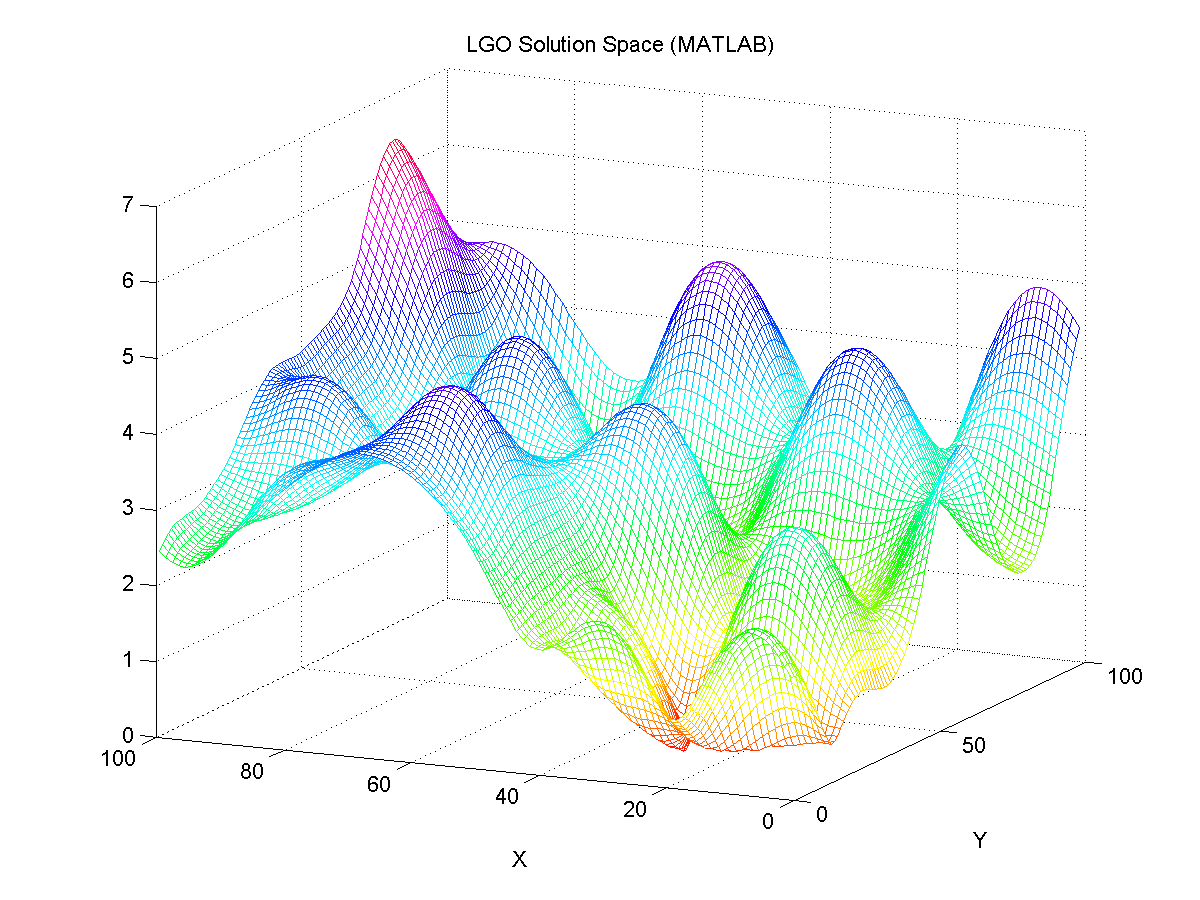
\includegraphics[scale=0.3]{figures/matlabgraph}
	\caption[MATLAB Plot]{Ein Plot aus dem Internet \cite{Plot}, der mit MATLAB erstellt wurde.}
	\label{fig:matlabfigur}
\end{figure}

\newpage
% !TEX root = ../maturaarbeit.tex
\chapter{Schluss}\label{chap:schluss}
\begin{enumerate}
	\item Kurze, prägnante Zusammenfassung der Ergebnisse, In-Beziehung-Stellen der Ergebnisse zur Einleitung
	\item Anregungen zur weiteren Vertiefung
Persönliche Bemerkungen: Schlussfolgerungen
	\item Welche neuen Erkenntnisse? Wo zeigten
sich besondere Schwierigkeiten? usw.
\end{enumerate}

\newpage

\appendix % <- Anhang
\listoffigures % <- Abbildungsverzeichnis
\listoftables  % <- Tabellenverzeichnis
% !TEX root = ../maturaarbeit.tex
\printbibliography[
heading=bibintoc,
title={Bibliography}
] % <- Literaturverzeichnis

\end{document}